\documentclass{article}
\usepackage[margin=1.5cm]{geometry}
\usepackage{amsmath}
\usepackage{amssymb}
\usepackage{graphicx}
\usepackage{tabls}
\usepackage{float}
\usepackage{tikz,tkz-graph}
\usepackage{enumitem}
\usepackage{empheQ_o}
\renewcommand{\baselinestretch}{1.4} 


\begin{document}

\begin{flushright}
Pablo Vaquer

NUEN 625 

Midterm

3/18/2016

\end{flushright}

The following 2 images clarify some of the notation I use for problems 1 and 2.

\begin{center}
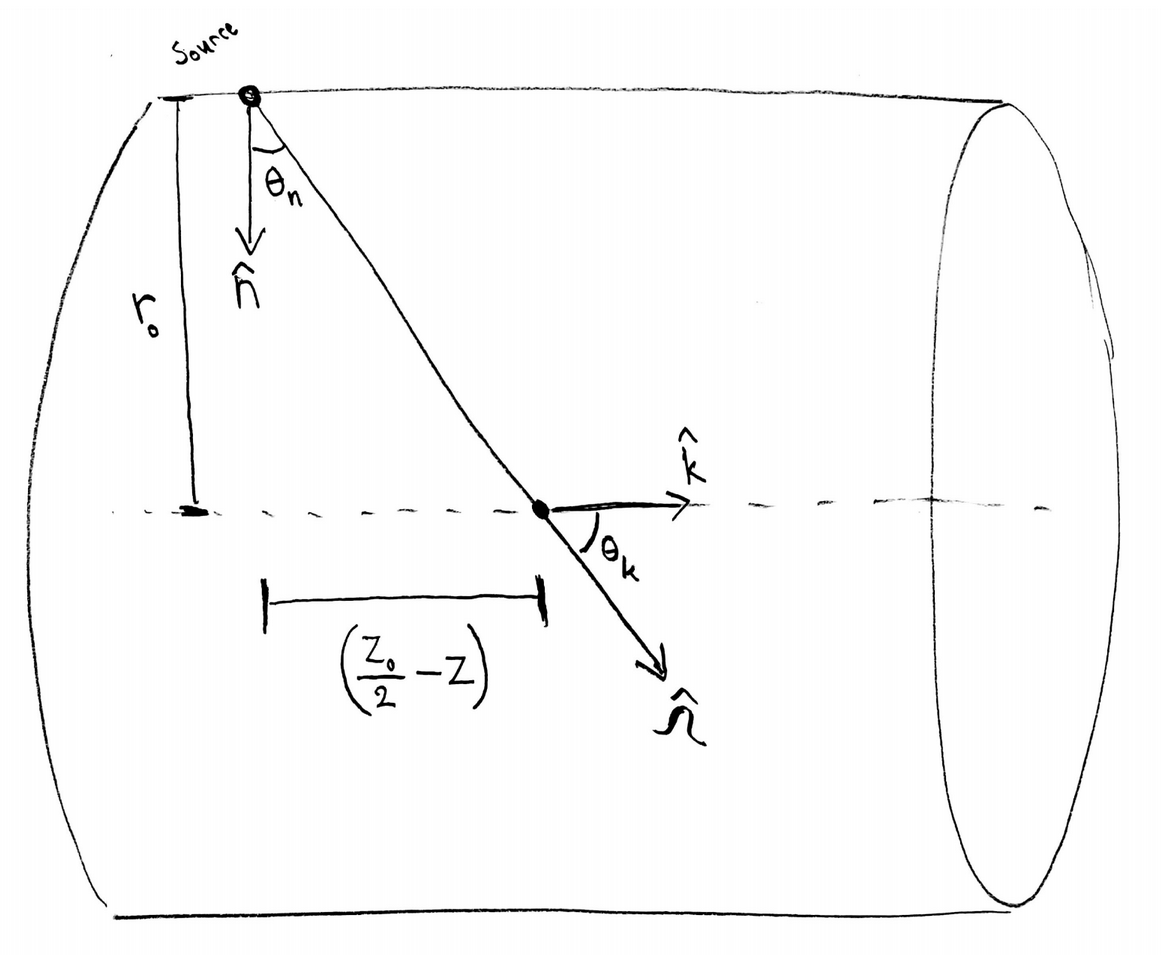
\includegraphics[width=0.66\textwidth]{midterm1.png}
\end{center}

\vspace{1cm}

\begin{center}
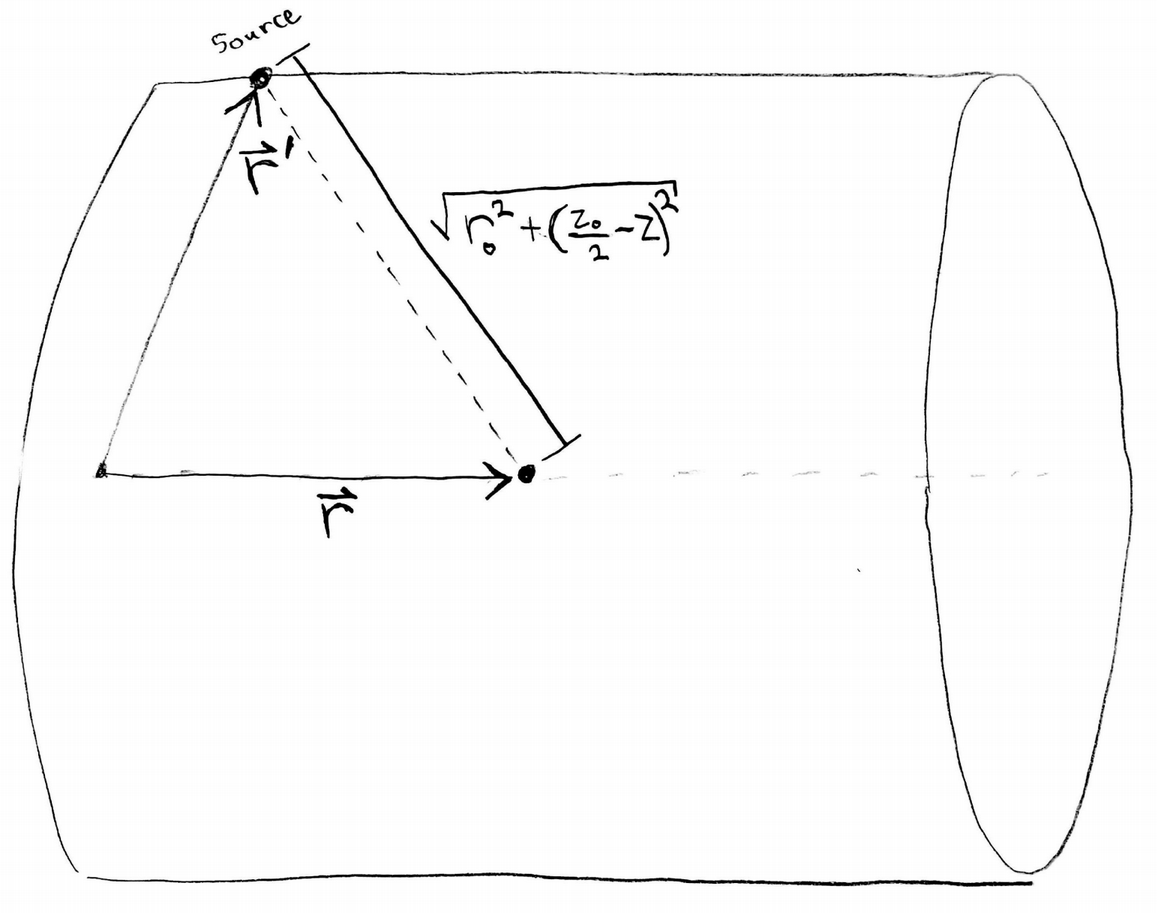
\includegraphics[width=0.66\textwidth]{midterm2.png}
\end{center}

\pagebreak

\section*{Problem 1}
\subsection*{(a)}

The general point kernal formula is 
\begin{equation*}
\phi(\vec{r}) = \int_V dV' \, \frac{Q(\vec{r}\,',\hat{\Omega})}{||\vec{r}\,'-\vec{r}||^2} \text{exp} \Big[ - \tau \big(\vec{r}\,', \vec{r} \big) \Big] \: .
\end{equation*}
Since there is no material attenuation and the source is a surface, the point kernal formula simplifies to  
\begin{equation}
\phi(\vec{r}) = \int_A dA' \, \frac{Q_o r_o}{4 \pi ||\vec{r}\,'-\vec{r}||^2} 
\end{equation}
where 
\begin{equation*}
||\vec{r}\,'-\vec{r}|| =  \sqrt{ r_o^2 + \big(\frac{z_o}{2}-z\big)^2 } 
\end{equation*}
and
\begin{equation*}
dA' = r_o d\varphi dz\: .
\end{equation*}
Thus,
\begin{equation*}
\phi\Big(\frac{z_o}{2}\Big) =\int_0^{z_o} dz \int_0^{2\pi} d\varphi \, \frac{Q_o r_o}{4 \pi \Big[ r_o^2 + \big(\frac{z_o}{2}-z\big)^2 \Big]} 
\end{equation*}
\begin{equation*}
\phi\Big(\frac{z_o}{2}\Big) =\int_0^{z_o} dz  \, \frac{Q_o r_o}{2 \Big[ r_o^2 + \big(\frac{z_o}{2}-z\big)^2 \Big]} 
\end{equation*}
\begin{equation*}
\phi\Big(\frac{z_o}{2}\Big) =\frac{Q_o}{2 r_o} \int_0^{z_o} dz  \, \frac{1}{ 1 + \Big(\frac{\frac{z_o}{2}-z}{r_o}\Big)^2} \: .
\end{equation*}
Now we can use $u$-substitution to solve the integral where
\begin{equation*}
u = \Big(\frac{\frac{z_o}{2}-z}{r_o}\Big)
\end{equation*}
\begin{equation*}
\frac{du}{dz} = -\frac{1}{r_o}
\end{equation*}
\begin{equation*}
dz = - r_o \, du \: .
\end{equation*}
This gives us that
\begin{equation*}
\phi\Big(\frac{z_o}{2}\Big) =-\frac{Q_o}{2} \text{arctan}\Big(\frac{\frac{z_o}{2}-z}{r_o}\Big)} \Big|_0^{z_o} 
\end{equation*}
\begin{equation*}
\phi\Big(\frac{z_o}{2}\Big) =-\frac{Q_o}{2} \Bigg[ \text{arctan}\Big(-\frac{z_o}{2r_o}\Big)} - \text{arctan}\Big(\frac{z_o}{2r_o}\Big)} \Bigg] 
\end{equation*}
\begin{equation*}
\boxed{ \phi\Big(\frac{z_o}{2}\Big) =Q_o \, \text{arctan}\Big(\frac{z_o}{2r_o}\Big) } \: .
\end{equation*}

\pagebreak

\subsection*{(b)}

Eq.(1) can be modified to calculate for the current by simply including a $(\hat{\Omega} \cdot \hat{k})$ term in the integrand, 
\begin{equation*}
J(\vec{r}) = \int_A dA' \, \frac{Q_o}{4 \pi ||\vec{r}\,'-\vec{r}||^2} (\hat{\Omega} \cdot \hat{k})
\end{equation*}
where 
\begin{equation*}
||\vec{r}\,'-\vec{r}|| =  \sqrt{ r_o^2 + \big(\frac{z_o}{2}-z\big)^2 } 
\end{equation*}
\begin{equation*}
(\hat{\Omega} \cdot \hat{k}) = \cos(\theta_k) = \frac{\frac{z_o}{2} - z}{\sqrt{ r_o^2 + \big(\frac{z_o}{2} - z\big)^2 } }
\end{equation*}
and
\begin{equation*}
dA' = r_o d\varphi dz \: .
\end{equation*}
Thus,
\begin{equation*}
J\Big(\frac{z_o}{2}\Big) = \frac{Q_o r_o}{4\pi} \int_0^{z_o} dz \int_0^{2\pi} d\varphi \, \frac{\frac{z_o}{2} - z}{\Big[ r_o^2 + \big(\frac{z_o}{2} - z\big)^2 \Big]^{\frac{3}{2}}} 
\end{equation*}
\begin{equation*}
J\Big(\frac{z_o}{2}\Big) = \frac{Q_o r_o}{2} \int_0^{z_o} dz \, \frac{\frac{z_o}{2} - z}{\Big[ r_o^2 + \big(\frac{z_o}{2} - z\big)^2 \Big]^{\frac{3}{2}}} 
\end{equation*}
Now we can use $u$-substitution to solve the integral where
\begin{equation*}
u = r_o^2 + \big(\frac{z_o}{2}-z \big)^2
\end{equation*}
\begin{equation*}
\frac{du}{dz} = -2 \big(\frac{z_o}{2}-z \big)
\end{equation*}
\begin{equation*}
dz = - \frac{du}{2 \big(\frac{z_o}{2}-z \big)} \: .
\end{equation*}
This gives us that
\begin{equation*}
J\Big(\frac{z_o}{2}\Big) = - \frac{Q_o r_o}{4} \int_{r_o^2+(\frac{z_o}{2})^2}^{r_o^2+(-\frac{z_o}{2})^2} dz \, u^{-\frac{3}{2}} 
\end{equation*}
\begin{equation*}
J\Big(\frac{z_o}{2}\Big) =\frac{Q_o r_o}{2} \Bigg[ \frac{1}{\sqrt{r_o^2+\big(-\frac{z_o}{2}\big)^2}} - \frac{1}{\sqrt{r_o^2+\big(\frac{z_o}{2}\big)^2}} \Bigg] 
\end{equation*}
\begin{equation*}
\boxed{ J\Big(\frac{z_o}{2}\Big) = 0 } \: .
\end{equation*}

\pagebreak

\subsection*{(c)}

The general point kernal formula is 
\begin{equation*}
\phi(\vec{r}) = \int_V dV' \, \frac{Q(\vec{r}\,',\hat{\Omega})}{||\vec{r}\,'-\vec{r}||^2} \text{exp} \Big[ - \tau \big(\vec{r}\,', \vec{r} \big) \Big] \: .
\end{equation*}
Since there is no material attenuation and the source is a surface, the point kernal formula simplifies to  
\begin{equation}
\phi(\vec{r}) = \int_A dA' \, \frac{Q_o r_o}{4 \pi ||\vec{r}\,'-\vec{r}||^2} 
\end{equation}
where 
\begin{equation*}
||\vec{r}\,'-\vec{r}|| =  \sqrt{ r_o^2 + \big(z_o-z\big)^2 } 
\end{equation*}
and
\begin{equation*}
dA' = r_o d\varphi dz \: .
\end{equation*}
Thus,
\begin{equation*}
\phi(z_o) =\int_0^{z_o} dz \int_0^{2\pi} d\varphi \, \frac{Q_o r_o}{4 \pi \Big[ r_o^2 + \big(z_o-z\big)^2 \Big]} 
\end{equation*}
\begin{equation*}
\phi(z_o) =\int_0^{z_o} dz  \, \frac{Q_o r_o}{2 \Big[ r_o^2 + \big(z_o-z\big)^2 \Big]} 
\end{equation*}
\begin{equation*}
\phi(z_o) =\frac{Q_o}{2 r_o} \int_0^{z_o} dz  \, \frac{1}{ 1 + \Big(\frac{z_o-z}{r_o}\Big)^2} \: .
\end{equation*}
Now we can use $u$-substitution to solve the integral where
\begin{equation*}
u = \Big(\frac{z_o-z}{r_o}\Big)
\end{equation*}
\begin{equation*}
\frac{du}{dz} = - \frac{1}{r_o}
\end{equation*}
\begin{equation*}
dz = - r_o \, du \: .
\end{equation*}
This gives us that
\begin{equation*}
\phi(z_o) =-\frac{Q_o}{2} \text{arctan}\Big(\frac{z_o-z}{r_o}\Big)} \Big|_0^{z_o} 
\end{equation*}
\begin{equation*}
\phi(z_o) =-\frac{Q_o}{2} \Bigg[ \text{arctan}(0)} - \text{arctan}\Big(\frac{z_o}{r_o}\Big)}\Bigg] 
\end{equation*}
\begin{equation*}
\boxed{ \phi(z_o) =\frac{Q_o}{2} \text{arctan}\Big(\frac{z_o}{r_o}\Big) } \: .
\end{equation*}

\pagebreak

\subsection*{(d)}

Eq.(2) can be modified to calculate for the current by simply including a $(\hat{\Omega} \cdot \hat{k})$ term in the integrand, 
\begin{equation*}
J(\vec{r}) = \int_A dA' \, \frac{Q_o r_o}{4 \pi ||\vec{r}\,'-\vec{r}||^2} (\hat{\Omega} \cdot \hat{k})
\end{equation*}
where 
\begin{equation*}
||\vec{r}\,'-\vec{r}|| =  \sqrt{ r_o^2 + \big(z_o-z\big)^2 } 
\end{equation*}
\begin{equation*}
(\hat{\Omega} \cdot \hat{k}) = \cos(\theta_k) = \frac{z_o - z}{\sqrt{ r_o^2 + \big(z_o - z\big)^2 } }
\end{equation*}
and
\begin{equation*}
dA' = r_o d\varphi dz \: .
\end{equation*}
Thus,
\begin{equation*}
J\Big(z_o\Big) = \frac{Q_o r_o}{4\pi} \int_0^{z_o} dz \int_0^{2\pi} d\varphi \, \frac{z_o - z}{\Big[ r_o^2 + \big(z_o - z\big)^2 \Big]^{\frac{3}{2}}} 
\end{equation*}
\begin{equation*}
J\Big(z_o\Big) = \frac{Q_o r_o}{2} \int_0^{z_o} dz \, \frac{z_o - z}{\Big[ r_o^2 + \big(z_o - z\big)^2 \Big]^{\frac{3}{2}}} 
\end{equation*}
Now we can use $u$-substitution to solve the integral where
\begin{equation*}
u = r_o^2 + \big(z_o-z \big)^2
\end{equation*}
\begin{equation*}
\frac{du}{dz} = -2 \big(z_o-z \big)
\end{equation*}
\begin{equation*}
dz = - \frac{du}{2 \big(z_o-z \big)} \: .
\end{equation*}
This gives us that
\begin{equation*}
J\Big(z_o\Big) = - \frac{Q_o r_o}{4} \int_{r_o^2+z_o^2}^{r_o^2} dz \, u^{-\frac{3}{2}} 
\end{equation*}
\begin{equation*}
J\Big(z_o\Big) = \frac{Q_o r_o}{2} \Bigg( \frac{1}{\sqrt{r_o^2}} - \frac{1}{\sqrt{r_o^2+z_o^2}} \Bigg) 
\end{equation*}
\begin{equation*}
\boxed{ J\Big(z_o\Big) = \frac{Q_o}{2} \Bigg( 1 - \frac{r_o}{\sqrt{r_o^2+z_o^2}} \Bigg) } 
\end{equation*}

\pagebreak

\section*{Problem 2}
\subsection*{(a)}

The general point kernal formula is 
\begin{equation*}
\phi(\vec{r}) = \int_V dV' \, \frac{Q(\vec{r}\,',\hat{\Omega})}{||\vec{r}\,'-\vec{r}||^2} \text{exp} \Big[ - \tau \big(\vec{r}\,', \vec{r} \big) \Big] \: .
\end{equation*}
Since there is no material attenuation and the source is a surface, the point kernal formula simplifies to  
\begin{equation}
\phi(\vec{r}) = \int_A dA' \, \frac{Q_o}{4 \pi ||\vec{r}\,'-\vec{r}||^2} (\hat{\Omega} \cdot \hat{n})
\end{equation}
where 
\begin{equation*}
||\vec{r}\,'-\vec{r}|| =  \sqrt{  r_o^2 + \big(\frac{z_o}{2} -z \big)^2 } 
\end{equation*}
\begin{equation*}
(\hat{\Omega} \cdot \hat{n}) = \cos(\theta_n) = \frac{r_o}{\sqrt{ r_o^2 + \big(\frac{z_o}{2} -z \big)^2 } }
\end{equation*}
and
\begin{equation*}
dA' = r_o d\varphi dz \: .
\end{equation*}
Thus,
\begin{equation*}
\phi\Big(\frac{z_o}{2}\Big) =\int_0^{z_o} dz \int_0^{2\pi} d\varphi \, \frac{Q_o r_o^2}{4 \pi \Big[ r_o^2 + \big(\frac{z_o}{2}-z\big)^2 \Big]^{\frac{3}{2}}} 
\end{equation*}

\begin{equation*}
\phi\Big(\frac{z_o}{2}\Big) =\int_0^{z_o} dz  \, \frac{Q_o r_o^2}{2 \Big[ r_o^2 + \big(\frac{z_o}{2}-z\big)^2 \Big]^{\frac{3}{2}}} 
\end{equation*}

\begin{equation*}
\phi\Big(\frac{z_o}{2}\Big) = \frac{Q_o \big(z-\frac{z_o}{2}\big)}{2 \sqrt{ r_o^2 + \big(\frac{z_o}{2}-z\big)^2 }} \Big|_0^{z_o}
\end{equation*}

\begin{equation*}
\phi\Big(\frac{z_o}{2}\Big) = \frac{Q_o \frac{z_o}{2}}{2 \sqrt{ r_o^2 + \big(-\frac{z_o}{2}\big)^2 }} - \frac{Q_o \big(- \frac{z_o}{2}\big)}{2 \sqrt{ r_o^2 + \big(\frac{z_o}{2}\big)^2 }} 
\end{equation*}

\begin{equation*}
\phi\Big(\frac{z_o}{2}\Big) = \frac{Q_o \frac{z_o}{2} + Q_o \frac{z_o}{2}}{2 \sqrt{ r_o^2 + \big(\frac{z_o}{2}\big)^2 }} 
\end{equation*}

\begin{equation*}
\boxed{ \phi\Big(\frac{z_o}{2}\Big) = \frac{Q_o z_o}{2 \sqrt{ r_o^2 + \big(\frac{z_o}{2}\big)^2 }} } \: .
\end{equation*}

\pagebreak

\subsection*{(b)}

Eq.(3) can be modified to calculate for the current by simply including a $(\hat{\Omega} \cdot \hat{k})$ term in the integrandm, 
\begin{equation*}
J(\vec{r}) = \int_A dA' \, \frac{Q_o}{4 \pi ||\vec{r}\,'-\vec{r}||^2}  (\hat{\Omega} \cdot \hat{n}) (\hat{\Omega} \cdot \hat{k})
\end{equation*}
where 
\begin{equation*}
||\vec{r}\,'-\vec{r}|| =  \sqrt{ r_o^2 + \big(\frac{z_o}{2} - z\big)^2 } 
\end{equation*}
\begin{equation*}
(\hat{\Omega} \cdot \hat{n}) = \cos(\theta_n) = \frac{r_o}{\sqrt{ r_o^2 + \big(\frac{z_o}{2} -z \big)^2 } }
\end{equation*}
\begin{equation*}
(\hat{\Omega} \cdot \hat{k}) = \cos(\theta_k) = \frac{\frac{z_o}{2} - z}{\sqrt{ r_o^2 + \big(\frac{z_o}{2} - z\big)^2 } }
\end{equation*}
and
\begin{equation*}
dA' = r_o d\varphi dz \: .
\end{equation*}
Thus,
\begin{equation*}
J\Big(\frac{z_o}{2}\Big) =\int_0^{z_o} dz \int_0^{2\pi} d\varphi \, \frac{Q_o r_o^2 \big(\frac{z_o}{2} - z\big)}{4 \pi \Big[ r_o^2 + \big(\frac{z_o}{2}-z\big)^2 \Big]^2} 
\end{equation*}

\begin{equation*}
J\Big(\frac{z_o}{2}\Big) =\int_0^{z_o} dz  \, \frac{Q_o r_o^2 \big(\frac{z_o}{2} - z\big)}{2 \Big[ r_o^2 + \big(\frac{z_o}{2}-z\big)^2 \Big]^2} 
\end{equation*}

Now we can use $u$-substitution to solve the integral where
\begin{equation*}
u = r_o^2 + \big(\frac{z_o}{2}-z \big)^2
\end{equation*}
\begin{equation*}
\frac{du}{dz} = -2 \big(\frac{z_o}{2}-z \big)
\end{equation*}
\begin{equation*}
dz = - \frac{du}{2 \big(\frac{z_o}{2}-z \big)} \: .
\end{equation*}
This gives us that

\begin{equation*}
J\Big(\frac{z_o}{2}\Big) = \frac{Q_o r_o^2}{4 \Big[ r_o^2 + \big(\frac{z_o}{2}-z\big)^2 \Big]} \Big|_0^{z_o}
\end{equation*}

\begin{equation*}
J\Big(\frac{z_o}{2}\Big) = \frac{Q_o r_o^2}{4 \Big[ r_o^2 + \big(-\frac{z_o}{2}\big)^2 \Big]} - \frac{Q_o r_o^2}{4 \Big[ r_o^2 + \big(\frac{z_o}{2}\big)^2 \Big]} 
\end{equation*}

\begin{equation*}
\boxed{ J\Big(\frac{z_o}{2}\Big) = 0 } \: .
\end{equation*}

\pagebreak

\subsection*{(c)}

The general point kernal formula is 
\begin{equation*}
\phi(\vec{r}) = \int_V dV' \, \frac{Q(\vec{r}\,',\hat{\Omega})}{||\vec{r}\,'-\vec{r}||^2} \text{exp} \Big[ - \tau \big(\vec{r}\,', \vec{r} \big) \Big] \: .
\end{equation*}
Since there is no material attenuation and the source is a surface, the point kernal formula simplifies to  
\begin{equation}
\phi(\vec{r}) = \int_A dA' \, \frac{Q_o}{4 \pi ||\vec{r}\,'-\vec{r}||^2} (\hat{\Omega} \cdot \hat{n})
\end{equation}
where 
\begin{equation*}
||\vec{r}\,'-\vec{r}|| =  \sqrt{  r_o^2 + \big(z_o-z\big)^2 } 
\end{equation*}
\begin{equation*}
(\hat{\Omega} \cdot \hat{n}) = \cos(\theta_n) = \frac{r_o}{\sqrt{ r_o^2 + \big(z_o-z\big)^2 } }
\end{equation*}
and
\begin{equation*}
dA' = r_o d\varphi dz \: .
\end{equation*}
Thus,
\begin{equation*}
\phi(z_o) =\int_0^{z_o} dz \int_0^{2\pi} d\varphi \, \frac{Q_o r_o^2}{4 \pi \Big[ r_o^2 + \big(z_o-z\big)^2 \Big]^{\frac{3}{2}}} 
\end{equation*}

\begin{equation*}
\phi(z_o) =\int_0^{z_o} dz  \, \frac{Q_o r_o^2}{2 \Big[ r_o^2 + \big(z_o-z\big)^2 \Big]^{\frac{3}{2}}} 
\end{equation*}

\begin{equation*}
\phi(z_o) = \frac{Q_o \big(z-z_o\big)}{2 \sqrt{ r_o^2 + \big(z_o-z\big)^2 }} \Big|_0^{z_o}
\end{equation*}

\begin{equation*}
\boxed{ \phi(z_o) = \frac{Q_o  z_o}{2 \sqrt{ r_o^2 + z_o^2 }} } \: .
\end{equation*}

\pagebreak

\subsection*{(d)}

Eq.(4) can be modified to calculate for the current by simply including a $(\hat{\Omega} \cdot \hat{k})$ term in the integrand, 
\begin{equation*}
J(\vec{r}) = \int_A dA' \, \frac{Q_o}{4 \pi ||\vec{r}\,'-\vec{r}||^2}  (\hat{\Omega} \cdot \hat{n}) (\hat{\Omega} \cdot \hat{k})
\end{equation*}
where 
\begin{equation*}
||\vec{r}\,'-\vec{r}|| =  \sqrt{ r_o^2 + \big(z_o - z\big)^2 } 
\end{equation*}
\begin{equation*}
(\hat{\Omega} \cdot \hat{n}) = \cos(\theta_n) = \frac{r_o}{\sqrt{ r_o^2 + \big(z_o -z \big)^2 } }
\end{equation*}
\begin{equation*}
(\hat{\Omega} \cdot \hat{k}) = \cos(\theta_k) = \frac{z_o - z}{\sqrt{ r_o^2 + \big(z_o - z\big)^2 } }
\end{equation*}
and
\begin{equation*}
dA' = r_o d\varphi dz \: .
\end{equation*}
Thus,
\begin{equation*}
J\Big(\frac{z_o}{2}\Big) =\int_0^{z_o} dz \int_0^{2\pi} d\varphi \, \frac{Q_o r_o^2 \big(z_o - z\big)}{4 \pi \Big[ r_o^2 + \big(z_o-z\big)^2 \Big]^2} 
\end{equation*}

\begin{equation*}
J\Big(\frac{z_o}{2}\Big) =\int_0^{z_o} dz  \, \frac{Q_o r_o^2 \big(z_o - z\big)}{2 \Big[ r_o^2 + \big(z_o-z\big)^2 \Big]^2} 
\end{equation*}

Now we can use $u$-substitution to solve the integral where
\begin{equation*}
u = r_o^2 + \big(z_o-z \big)^2
\end{equation*}
\begin{equation*}
\frac{du}{dz} = -2 \big(z_o-z \big)
\end{equation*}
\begin{equation*}
dz = - \frac{du}{2 \big(z_o-z \big)} \: .
\end{equation*}
This gives us that

\begin{equation*}
J\Big(\frac{z_o}{2}\Big) = \frac{Q_o r_o^2}{4 \Big[ r_o^2 + \big(z_o-z\big)^2 \Big]} \Big|_0^{z_o}
\end{equation*}

\begin{equation*}
J\Big(\frac{z_o}{2}\Big) = \frac{Q_o r_o^2}{4 r_o^2} - \frac{Q_o r_o^2}{4 \big( r_o^2 + z_o^2 \big)} 
\end{equation*}

\begin{equation*}
\boxed{ J\Big(\frac{z_o}{2}\Big) = \frac{Q_o}{4} \Bigg(1 - \frac{r_o^2}{r_o^2 + z_o^2}\Bigg) } \: .
\end{equation*}

\pagebreak

\section*{Problem 3}
\subsection*{(a)}
The following diffusion equation 
\begin{equation*}
- \frac{\partial}{\partial x} \frac{1}{3\sigma_t} \frac{\partial \phi}{\partial x} + \sigma_a \phi = 0
\end{equation*} 
can be rewritten as
\begin{equation*}
\frac{\partial^2 \phi}{\partial x^2} - 3\sigma_t \sigma_a \phi = 0 \: .
\end{equation*} 
The solution to this equation for a semi-infinite medium is
\begin{equation}
\label{eq:phi_x}
\phi(x) = \phi_o e^{- \sqrt{3\sigma_t \sigma_a} \, x} 
\end{equation}
with a Mark boundary at $x=0$. Note that a Mark boundary condition is an approximation of the half-range current on a boundary using a linearly-anisotropic flux with the value of $\mu=-1/\sqrt{3}$ or $\mu=1/\sqrt{3}$ (depending on the boundary), such that 
\begin{equation*}
J^+ = 2\pi \int_0^1 d\mu \, \mu \psi \approx 2\pi \Big(\frac{1}{\sqrt{3}}\Big) \Bigg[ \frac{1}{4\pi} \phi + \frac{3}{4\pi} \Big(\frac{1}{\sqrt{3}}\Big) J \Bigg]\: .
\end{equation*}
Thus, if $J^+=1$ then 
\begin{equation*}
2\pi \Big(\frac{1}{\sqrt{3}}\Big) \Bigg[ \frac{1}{4\pi} \phi + \frac{3}{4\pi} \Big(\frac{1}{\sqrt{3}}\Big) J \Bigg] = 1 \
\end{equation*} 

\begin{equation*}
 \frac{1}{4\pi} \phi + \frac{\sqrt{3}}{4\pi} J = \frac{\sqrt{3}}{2\pi} \: .
\end{equation*}

\begin{equation*}
\phi + \sqrt{3} J = 2 \sqrt{3} 
\end{equation*}
and therefore
\begin{equation*}
\phi(0) - \sqrt{3} D \frac{\partial \phi(0)}{\partial x} = 2 \sqrt{3} 
\end{equation*}
\begin{equation*}
\phi_o - \frac{\sqrt{3}}{3\sigma_t} \big( - \sqrt{3 \sigma_t \sigma_a} \big) \phi_o = 2 \sqrt{3} 
\end{equation*}
\begin{equation*}
\phi_o \Big( 1 + \sqrt{\frac{\sigma_a}{\sigma_t}} \Big) = 2 \sqrt{3} 
\end{equation*}
\begin{equation}
\label{eq:phi_o}
\phi_o  =  \frac{2 \sqrt{3}}{1 + \sqrt{\frac{\sigma_a}{\sigma_t}}} \: .
\end{equation}
By plugging in Eq.(\ref{eq:phi_o}) into Eq.(\ref{eq:phi_x}),
\begin{equation*}
\phi (x)  =  \frac{2 \sqrt{3}\, \text{exp}(- \sqrt{3\sigma_t \sigma_a} \, x)}{1 + \sqrt{\frac{\sigma_a}{\sigma_t}}} \: . 
\end{equation*}

\vspace{0.5cm}

The fraction reflected is equal to $\alpha = J^- / J^+$ at $x=0$, where
\begin{equation*}
J^+ = 1 
\end{equation*} 
\begin{equation*}
J^- = \frac{1}{2\sqrt{3}} \big[\phi(0) - \sqrt{3}J(0) \big] \: .
\end{equation*}

\begin{equation*}
\alpha = \frac{1}{2\sqrt{3}} \Big[\phi_o + \frac{\sqrt{3}}{3\sigma_t}  \big( - \sqrt{3 \sigma_t \sigma_a} \big) \phi_o \Big]
\end{equation*}
\begin{equation*}
\alpha = \frac{1}{2\sqrt{3}} \phi_o \Big( 1- \sqrt{\frac{\sigma_a}{\sigma_t}} \Big)
\end{equation*}
and by combining this with Eq.(\ref{eq:phi_o}) we get
\begin{equation*}
\boxed{ \alpha = \Bigg( \frac{1 - \sqrt{\frac{\sigma_a}{\sigma_t}}}{1 + \sqrt{\frac{\sigma_a}{\sigma_t}}} \Bigg) }
\end{equation*}

\subsection*{(b)}
\begin{equation*}
\boxed{ \lim_{\sigma_a \to 0} \Bigg( \frac{1 - \sqrt{\frac{\sigma_a}{\sigma_t}}}{1 + \sqrt{\frac{\sigma_a}{\sigma_t}}} \Bigg) = 1 }
\end{equation*}

\subsection*{(c)}
\begin{equation*}
\boxed{ \lim_{\sigma_a \to \sigma_t} \Bigg( \frac{1 - \sqrt{\frac{\sigma_a}{\sigma_t}}}{1 + \sqrt{\frac{\sigma_a}{\sigma_t}}} \Bigg) = 0 }
\end{equation*}


\pagebreak

\section*{Problem 4}

In the weighted residual method 
\begin{equation*}
\int_{i-1/2}^{i+1/2} dx \, R(x) W_n(x) = 0 \: .
\end{equation*}
In this case the residual is 
\begin{equation*}
R(x) = \frac{\partial \tilde{f}}{\partial x} + \sigma \tilde{f} 
\end{equation*}
and thus
\begin{equation*}
\int_{x_{i-1/2}}^{x_{i+1/2}} dx \, \Big( \frac{\partial \tilde{f}}{\partial x} + \sigma \tilde{f}  \Big) W_n(x) = 0 \: .
\end{equation*}
The weight space generates two different equations. For $W_1$, 
\begin{equation*}
\int_{x_{i-1/2}}^{x_{i}} dx \, \Big( \frac{\partial \tilde{f}}{\partial x} + \sigma \tilde{f}  \Big) = 0 
\end{equation*}
and for $W_2$
\begin{equation*}
\int_{x_{i}}^{x_{i+1/2}} dx \, \Big( \frac{\partial \tilde{f}}{\partial x} + \sigma \tilde{f}  \Big)  = 0 \: .
\end{equation*}

Now, for $W_1$ we get
\begin{equation*}
\tilde{f} (x_{i}) - \tilde{f} (x_{i-1/2}) + \int_{x_{i-1/2}}^{x_{i}} dx \, \sigma \tilde{f} = 0   \: .
\end{equation*}
\begin{equation*}
\frac{f_L + f_R}{2} - 1 + \sigma f_L \frac{h_i}{2}  = 0 
\end{equation*}
\begin{equation*}
f_L + f_R - 2 + \sigma f_L h_i  = 0 
\end{equation*}
\begin{equation}
\label{eq:W1}
(1 + \sigma h_i) f_L + f_R = 2 \: .
\end{equation}

Now, for $W_2$ we get
\begin{equation*}
\tilde{f} (x_{i+1/2}) - \tilde{f} (x_{i}) + \int_{x_{i}}^{x_{i+1/2}} dx \, \sigma \tilde{f} = 0   \: .
\end{equation*}
\begin{equation*}
f_R - \frac{f_L + f_R}{2} + \sigma f_R \frac{h_i}{2}  = 0 
\end{equation*}
\begin{equation*}
f_R - f_L + \sigma f_R h_i  = 0 
\end{equation*}
\begin{equation}
\label{eq:W2}
-f_L + (1 + \sigma h_i) f_R = 0 \: .
\end{equation}

From Eq.(\ref{eq:W2}) we get
\begin{equation}
\label{eq:f_L}
f_L  = (1 + \sigma h_i) f_R \: .
\end{equation}
By plugging in Eq.(\ref{eq:f_L}) into Eq.(\ref{eq:W1}) we get
\begin{equation*}
(1 + \sigma h_i)^2 f_R + f_R = 2  
\end{equation*}
\begin{equation*}
f_R = \frac{2}{1 + (1 + \sigma h_i)^2}  
\end{equation*}
\begin{equation*}
f_R = \frac{2}{2 + 2 \sigma h_i + \sigma^2 h_i^2}  
\end{equation*}
which gives us that 
\begin{equation*}
f_L  = \frac{2(1 + \sigma h_i)}{2 + 2 \sigma h_i + \sigma^2 h_i^2} 
\end{equation*}
\begin{equation*}
f_L  = \frac{2 + 2 \sigma h_i}{2 + 2 \sigma h_i + \sigma^2 h_i^2}  \: .
\end{equation*}

\pagebreak

Thus, the discrete solution is

\begin{center}
\begin{tabular}{ |l c l| }
  \hline
  $\tilde{f} \: =$ & $1$ & for $x \in x_{i-1/2}$ \\
   & $\frac{2 + 2 \sigma h_i}{2 + 2 \sigma h_i + \sigma^2 h_i^2}$ & for $x \in (x_{i-1/2},x_{i})$\\
   & $\frac{2}{2 + 2 \sigma h_i + \sigma^2 h_i^2} $ & for $x \in (x_{i},x_{i+1/2}]$ \\
   & $\frac{2 + \sigma h_i}{2 + 2 \sigma h_i + \sigma^2 h_i^2}$ & for $x = x_{i}$ \\
  \hline
\end{tabular} \: .
\end{center} 

\pagebreak

\section*{Problem 5}

\subsection*{(a)} 
Using asymptotic scaling,
\begin{equation*}
\frac{\epsilon}{v} \frac{\partial \psi}{\partial t} + \mu \frac{\partial \psi}{\partial x} + \frac{\sigma}{\epsilon} \psi = \frac{\sigma}{4\pi \epsilon} g 
\end{equation*}
\begin{equation*}
\frac{\epsilon}{v} \frac{\partial g}{\partial t}  = \frac{\sigma}{\epsilon} (\phi - g) \: .
\end{equation*}
After multiplying by $\epsilon$,
\begin{equation*}
\frac{\epsilon^2}{v} \frac{\partial \psi}{\partial t} + \mu \epsilon \frac{\partial \psi}{\partial x} + \sigma \psi = \frac{\sigma}{4\pi} g 
\end{equation*}
\begin{equation*}
\frac{\epsilon^2}{v} \frac{\partial g}{\partial t}  = \sigma (\phi - g) \: .
\end{equation*}
Now by using a power series for $\psi$, 
\begin{equation*}
\psi = \psi^{(0)} + \epsilon \psi^{(1)} + \epsilon^2 \psi^{(2)} + ... 
\end{equation*}
we get that
\begin{multline*}
\frac{\epsilon^2}{v} \frac{\partial \big(\psi^{(0)} + \epsilon \psi^{(1)} + \epsilon^2 \psi^{(2)} + ... \big)}{\partial t} + \mu \epsilon \frac{\partial \big(\psi^{(0)} + \epsilon \psi^{(1)} + \epsilon^2 \psi^{(2)} + ... \big)}{\partial x} + \sigma \big( \psi^{(0)} + \epsilon \psi^{(1)} + \epsilon^2 \psi^{(2)} + ... \big) = \\ \frac{\sigma}{4\pi} \big( g^{(0)} + \epsilon g^{(1)} + \epsilon^2 g^{(2)} + ... \big) \: 
\end{multline*}

\begin{equation*}
\frac{\epsilon^2}{v} \frac{\partial \big( g^{(0)} + \epsilon g^{(1)} + \epsilon^2 g^{(2)} + ... \big)}{\partial t} = \sigma \Big[ \big( \psi^{(0)} + \epsilon \psi^{(1)} + \epsilon^2 \psi^{(2)} + ... \big) - \big( g^{(0)} + \epsilon g^{(1)} + \epsilon^2 g^{(2)} + ... \big)  \Big] \: .
\end{equation*}

\vspace{0.5cm}

Now by keeping only the terms of order 1,
\begin{equation}
\label{eq:lead}
\boxed{ \psi^{(0)} =  \frac{1}{4\pi} g^{(0)} } 
\end{equation}

\subsection*{(b)}

Note that $g(x,t)$ is not a function of $\mu$ therefore using from Eq.(\ref{eq:lead}) we get,
\begin{equation}
J^{(0)} = 0 \: .
\end{equation}

\vspace{0.5cm}

Now, by keeping only the terms of order $\epsilon$,
\begin{equation}
\label{eq:e^1}
\mu \frac{\partial \psi^{(0)} }{\partial x} + \sigma \psi^{(1)}  =  \frac{1}{4\pi} \sigma g^{(1)} 
\end{equation}
\begin{equation*}
0 = \sigma ( \phi^{(1)} - g^{(1)} )  
\end{equation*}
By substituting Eq.(\ref{eq:lead}) into Eq.(\ref{eq:e^1}),
\begin{equation*}
\frac{\mu}{4\pi} \frac{\partial g^{(0)} }{\partial x} + \sigma \psi^{(1)}  =  \frac{1}{4\pi} \sigma g^{(1)} 
\end{equation*}
\begin{equation*}
\psi^{(1)}  = - \frac{\mu}{4\pi\sigma} \frac{\partial g^{(0)} }{\partial x} + \frac{1}{4\pi} g^{(1)} 
\end{equation*}
by multiplying by $\mu$ and integrating over all $4\pi$ steradians, 
\begin{equation}
\label{eq:J}
J^{(1)} = -\frac{1 }{3\sigma} \frac{\partial g^{(0)} }{\partial x}  \: .
\end{equation}

Now, by keeping only the terms of order $\epsilon^2$,
\begin{equation}
\label{eq:e^2}
\frac{1}{v} \frac{\partial \psi^{(0)}}{\partial t} + \mu \frac{\partial \psi^{(1)} }{\partial x} + \sigma \psi^{(2)}  =  \frac{\sigma}{4\pi} g^{(2)} 
\end{equation}
\begin{equation}
\label{eq:g}
\frac{1}{v} \frac{\partial  g^{(0)}}{\partial t}  = \sigma ( \phi^{(2)} - g^{(2)} )  \: .
\end{equation}
Now by integrating Eq.(\ref{eq:e^2}) over all $4\pi$ steradians
\begin{equation*}
\frac{1}{v} \frac{\partial \phi^{(0)}}{\partial t} + \frac{\partial J^{(1)} }{\partial x} + \sigma \phi^{(2)} =  \sigma g^{(2)} 
\end{equation*}
\begin{equation*}
\frac{1}{v} \frac{\partial \phi^{(0)}}{\partial t} + \frac{\partial J^{(1)} }{\partial x} + \sigma (\phi^{(2)} - \sigma g^{(2)}) = 0
\end{equation*}
and combining it with Eq.(\ref{eq:g})
\begin{equation*}
\frac{1}{v} \frac{\partial \phi^{(0)}}{\partial t} + \frac{\partial J^{(1)} }{\partial x} + \frac{1}{v} \frac{\partial  g^{(0)}}{\partial t} = 0 \: .
\end{equation*}
By integrating equation Eq.(\ref{eq:lead}) and substituting for $\phi^{(0)}$,
\begin{equation*}
\frac{1}{v} \frac{\partial g^{(0)}}{\partial t} + \frac{\partial J^{(1)} }{\partial x} + \frac{1}{v} \frac{\partial  g^{(0)}}{\partial t} = 0 
\end{equation*}
\begin{equation*}
\frac{2}{v} \frac{\partial g^{(0)}}{\partial t} + \frac{\partial J^{(1)} }{\partial x} = 0 
\end{equation*}
and by combining this with Eq.(\ref{eq:J}) we get a diffusion equation for $g^{(0)}$,
\begin{equation*}
\boxed{ \frac{2}{v} \frac{\partial g^{(0)}}{\partial t} - \frac{\partial}{\partial x} \Big(\frac{1 }{3\sigma} \frac{\partial g^{(0)} }{\partial x} \Big) = 0 } \: .
\end{equation*}



\end{document}




